\documentclass[../Thesis.tex]{subfiles}
\graphicspath{{\subfix{../figures/}}}
\begin{document}

\chapter{
    Data
}

The data used consists of six cycles. This means that the total data set consists of six simulation runs. However, each of the runs contains many batches in sequence. The following table lists the number of batches in each of the simulations and some basic statistics

\begin{table}[h]
    \centering
    \begin{tabular}{c|c|c|c}
        Cycle & \#batch & $\mu_{batch}$ & $\sigma^2_{batch}$\\ \hline
        A & 66 & 14.776 & 3.641\\
        B & 64 & 15.644 & 3.915\\
        C & 61 & 17.714 & 2.330\\
        D & 60 & 18.069 & 6.922\\
        E & 60 & 18.088 & 9.613\\
        F & 63 & 17.227 & 7.766
    \end{tabular}
    \caption{Per cycle batch statistics}
    \label{tab:cycle basi stats}
\end{table}

Each batch is comprised several states. These include adding materials (IDs 1 through 4), centrifugation (ID 5), product transfer (the precipitate generated from the centrifugation, ID 6), chemical reaction (ID 7), a post operation state (\textcolor{red}{Probably to let it cool down to a point where it is ready for further processing}, ID 8), Cooling of the product (ID 9), material transfer (transfer the gained product before cleaning of the reaction vessel and/or prepare for the next reaction batch, ID 10).


\section{Cleaning operations}
Sometimes, the vessel is cleansed. This is however not every time after a batch so might be interesting to investigate further. Initially, per cycle, the cleanings are summarized in the following table with basic statistics. As can be seen, there is quite some differences.

The most notifiable differences per batch are the number of cleanses especially when comparing to table \ref{tab:cycle basi stats}. For the first two cycles, the cleanses seem to be in between every batch, which is indeed also the while the later four are only sometimes. Furthermore, although the cleanses are between every batch for cycles A and B, the variances are extremely different. For the last four cycles, they seem to be grouped further, E and F are very alike while cleanses in C and D are generally longer although D has a substantially smaller variance than C.

\begin{table}[h]
    \centering
    \begin{tabular}{c|c|c|c|c|c}
        Cycle & \#ops & min & max & $\mu$ & $\sigma^2$\\ \hline
        A & 65 & 1.113 & 3.067 & 1.917 & 0.269\\
        B & 63 & 1.324 & 1.751 & 1.566 & 0.00883\\
        C & 9  & 1.544 & 3.306 & 2.153 & 0.277\\
        D & 10 & 1.474 & 2.009 & 1.581 & 0.0212\\
        E & 10 & 0.827 & 1.584 & 1.465 & 0.0462\\
        F & 10 & 0.748 & 1.610 & 1.466 & 0.0595
    \end{tabular}
    \caption{Per cycle cleansing statistics}
    \label{tab:cycle cleansing stats stats}
\end{table}

To verify these observations and potentially discovering more important facts of their probability distributions, histograms are plotted in the following figure \ref{fig:cycle cleaning histograms}. We indeed again observe the likeliness between the cycles A and B, C and D, E and F respectively. Also, for the first two cycles and more so cycle B, the cleaning times are somewhat normally distributed although cycle A has a very heavy right tail in that case. The later four cycles only have 10 observations but the mode (i.e. peak) seem to be about the same.

\begin{figure}[h]
    \centering
    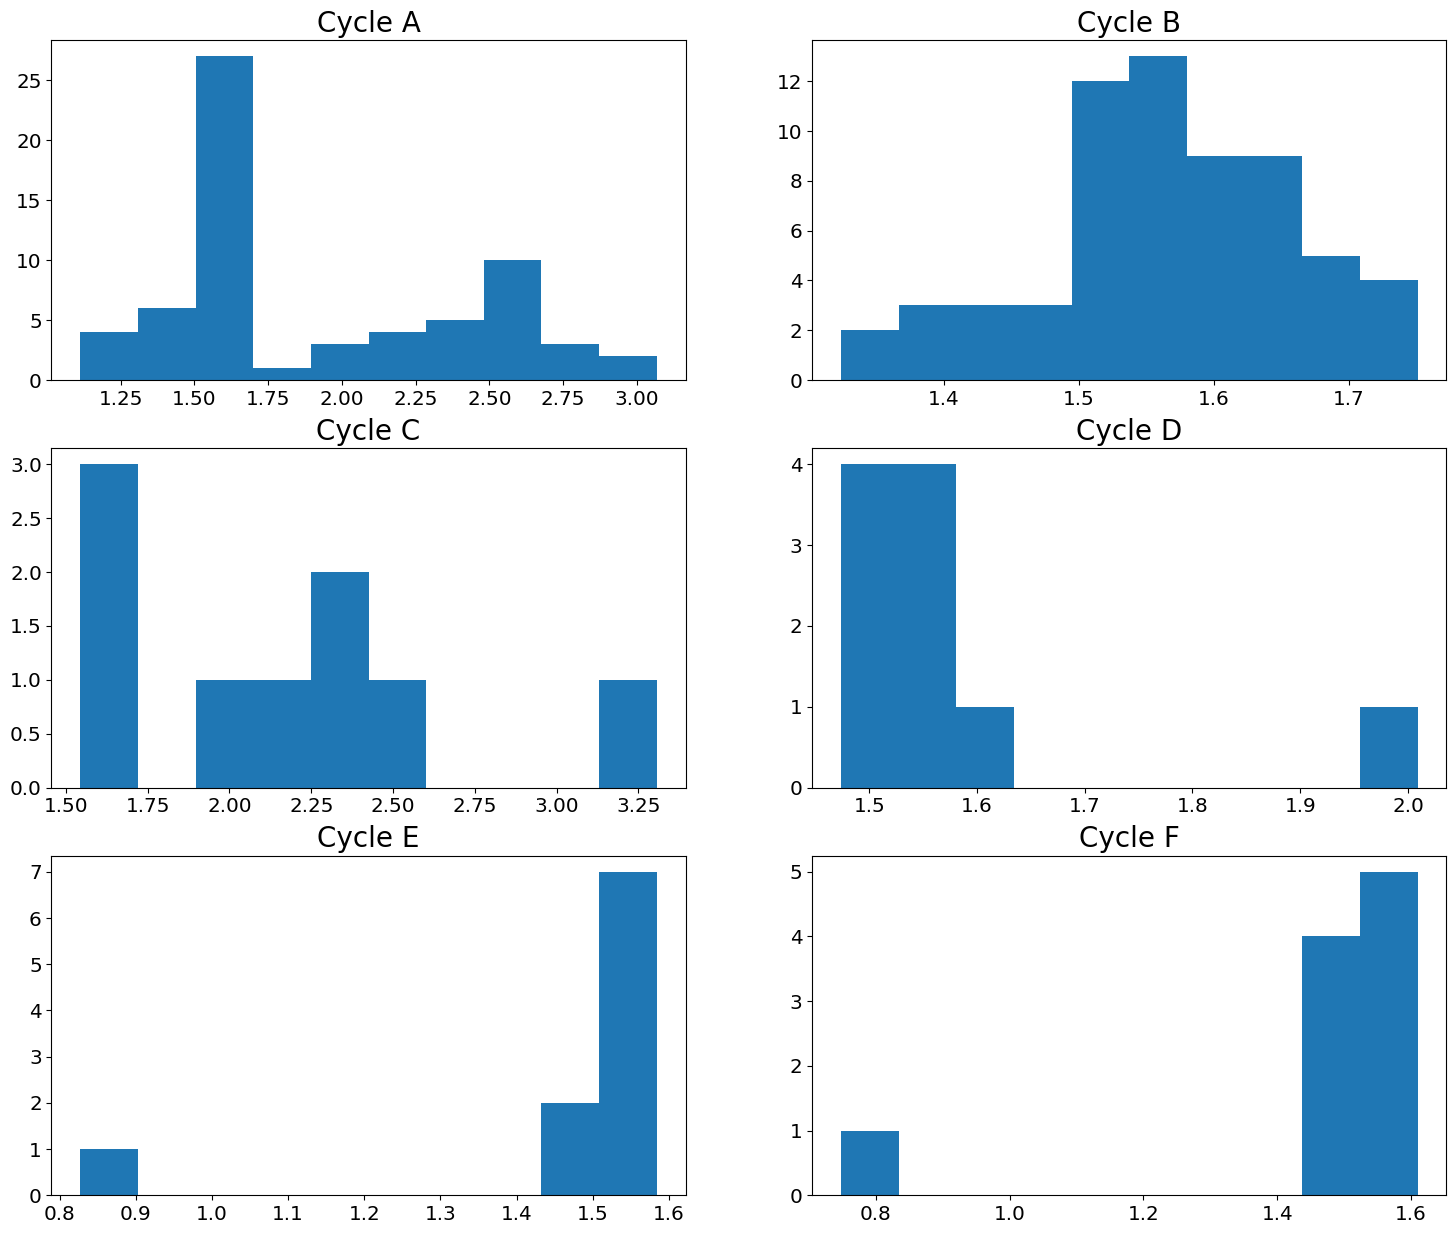
\includegraphics[width=0.8\linewidth]{figures/Multiple cycles data/Cleaning batches histograms.png}
    \caption{Each of the 6 cycles, cleaning operations histograms.}
    \label{fig:cycle cleaning histograms}
\end{figure}

From the above observation of like modes one may want to observe the histogram of the combined set of cleaning times. In particular, under the hypothesis that the durations are actually from the same probability distributions and realized independently within each cycle a histogram of all the observations are of interest and is shown in figure \ref{fig:cycle cleaning histograms combined} below.


\begin{figure}[H]
    \centering
    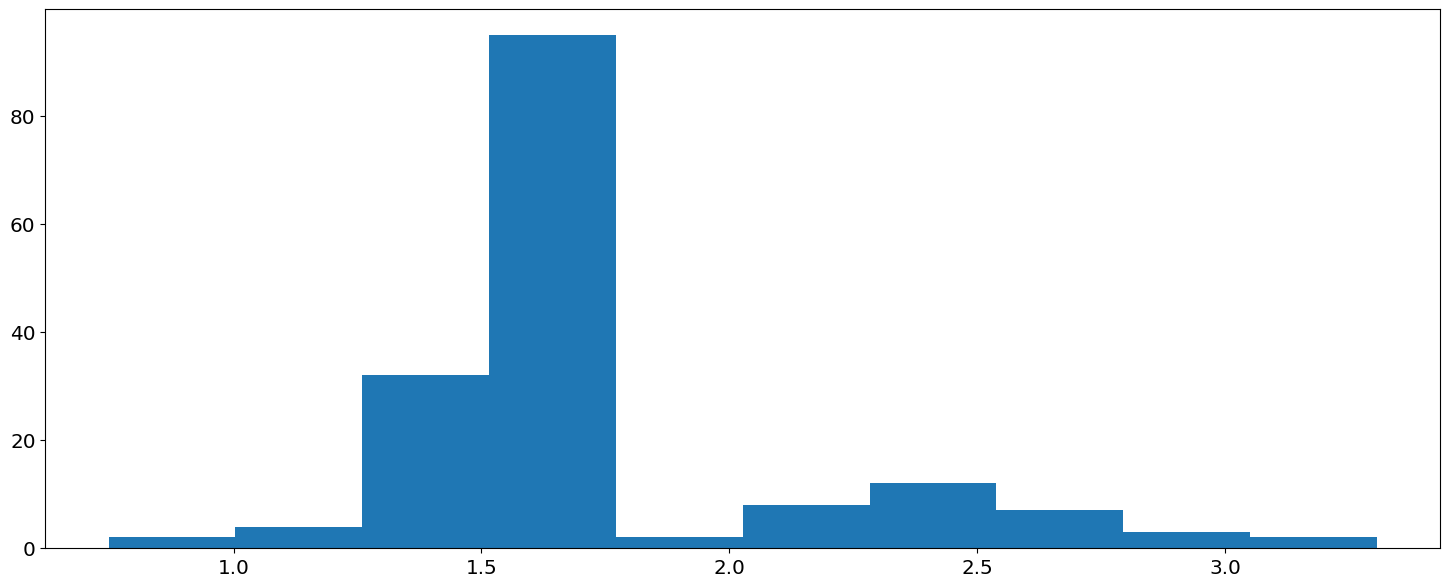
\includegraphics[width=0.8\linewidth]{figures/Multiple cycles data/Cleaning batches histograms combined.png}
    \caption{Combined cleaning operations histograms.}
    \label{fig:cycle cleaning histograms combined}
\end{figure}


Finally, to get a better overview of the irregularities is the number of cleaning periods (mostly concerning cycles C through F), each cleaning operation is shown in the following figure \ref{fig:cycle cleaning time series}. The vertical shaded rectangles signify the period in which a cleaning operation is taking place. Furthermore, the event IDs are shown but to get a clearer view on what is going on, a single rectangle (zoomed in) is shown in figure \ref{fig:cycle cleaning time series single}.

\begin{figure}[H]
    \centering
    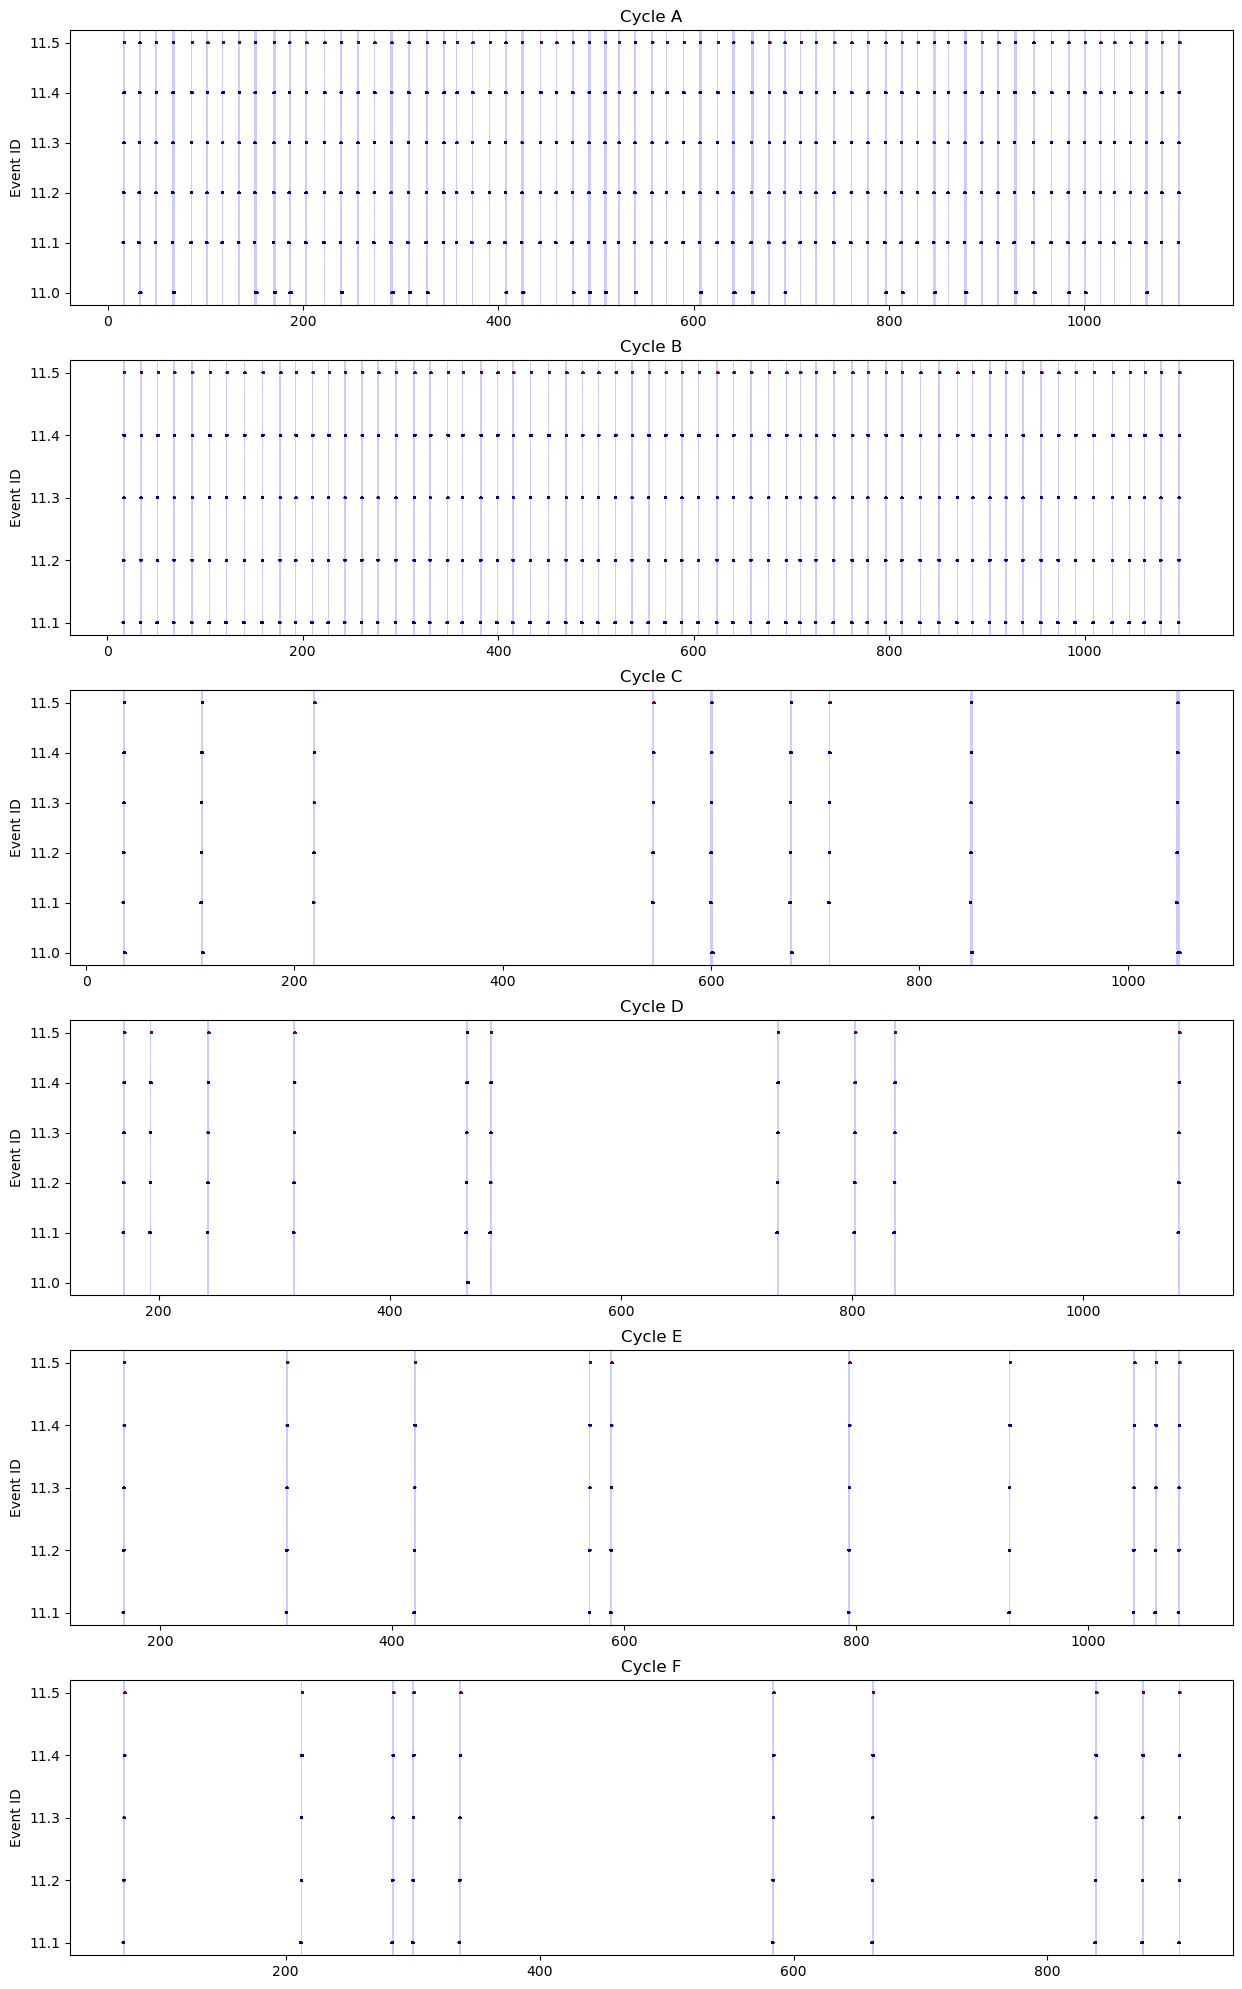
\includegraphics[width=0.9\linewidth]{figures/Multiple cycles data/Cleaning batches.png}
    \caption{Each of the 6 cycles, cleaning (corresponding to \texttt{BatchID = 0}). Each \textit(Cleaning Procedure), CIP, is highlighted with an opaque interval (the blue rectangles). The dots marked with red (only ID 11.5, but not all of these are red), is if the Cleaning ID is 0.}
    \label{fig:cycle cleaning time series}
\end{figure}


\begin{figure}[h]
    \centering
    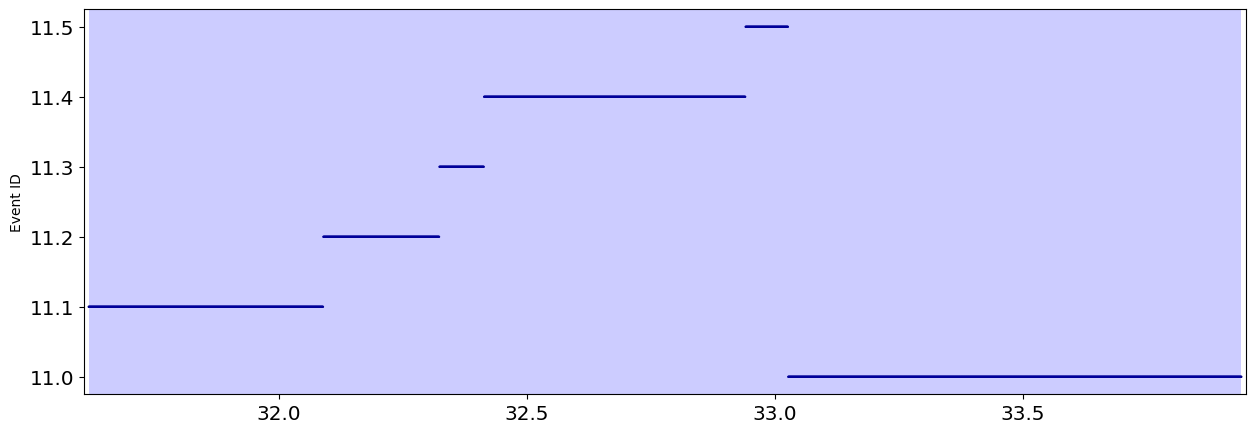
\includegraphics[width=0.9\linewidth]{figures/Multiple cycles data/Cleaning batches timeseries single.png}
    \caption{A single blue rectangle zoomed in}
    \label{fig:cycle cleaning time series single}
\end{figure}

It is observed that the observations marked with red in figure \ref{fig:cycle cleaning time series} occur exactly when that specific cleaning operation does not go to the state 11.0 after the flush of the tank (event ID 11.5) and vice versa. It is hard to conclude what this may mean, but the cleaning being in state 11.0 may indicate that the system is idle before continuing the next batch like what is observed from the other steps of the process flow. Also, it is noted that while the red dots occur nothing else is happening according to the dataset.


% There is a relationship between the red dots and when the cleaning does not \textit{return} to state 11.0


\end{document}
